\chapter{Introduction}
\label{chap:introduction}

In this chapter, I first discuss general research goals, lay out the structure of the thesis and summarise research contributions. The remainder of the chapter is devoted to background research about how to deal with data labelling, and in particular, data labelling for visual recognition. I then identify and discuss a set of projects and research strongly related to this work. 


\section{Research goals}
\label{sec:research_goals}

The central thesis of this dissertation is that annotation of data is best performed as a collaboration between human and a machine learning algorithm, known as \emph{human-in-the-loop} machine learning. The primary focus is a form which I term \gls{VBA}, where a machine learning model is trained interactively, based on verifying and correcting predictions from the model. As the model improves, the amount of correction required from a human annotator becomes less and less. 

The topic of this thesis arose due to frustration with the difficulty in capturing and labelling images for visual recognition tasks. Initially, segmentation was chosen, with exploratory work in assisted annotation and incremental training (Chapter~\ref{chap:bootstrap}). The remainder of the thesis is devoted to experimentation using system built specifically for \gls{VBA} using a \gls{CNN} based object detector.

Most machine learning tools focus on large scale visual recognition by collecting and annotating large datasets (for example with crowdsourcing) and training on large datasets. In this work, I focused on relatively small scale datasets, and the use of ideas around interactive annotation to create practical tools for rapidly prototyping new machine based tools. I aimed to address practical problems found along the way, such as the limited memory available for processing high-resolution images and evaluate as to how the quantity and quality of annotated data impacts on recognition performance and the flow-on influence on annotation performance in such a system.

\subsection {Thesis structure} 

% The first chapters of this thesis stand alone. In Chapter~\ref{chap:focus}, I look at the effect of cropping and resolution on image classification, and in Chapter~\ref{chap:metric} I experiment with a new method of metric learning, for instance, recognition, a form of n-way siamese network. 

% The rest of the thesis from Chapter~\ref{chap:bootstrap} onward is devoted to the central topic of the thesis, \gls{VBA}. 

In Chapter~\ref{chap:bootstrap}, I explore its application to image segmentation where image masks from a model are corrected with a set of drawing tools. I explore several angles for assisted image annotation and conclude that the verification based process is the most promising. Contrary to popular belief that \gls{CNN}s require much data and much training time, I demonstrate the opposite,  using few images and also very little training time whereby a \gls{CNN} can be trained to a level that provides genuine assistance to a human annotator. 

Chapter~\ref{chap:design} is devoted to the design and implementation of a \gls{VBA} system for object detection. I describe the goals, usage and implementation of a web-based tool created for this work. Some ideas implemented for this work are discussed, including a machine-assisted method of reviewing and verifying existing annotations, and the use of a dual threshold to make best use of weak detections without overwhelming the user.

In Chapter~\ref{chap:object_detection}, I describe the object detection \gls{CNN} model used in this work, the object detection background behind it, and implementation differences in this work from the model and training method described in the literature. I propose a variety of methods specifically for improving the object detector to make the best use of limited data, these include methods of training and inference for high-resolution images, methods for incremental training online and cyclical learning rate scheduling. Finally, I present a study investigating how noise levels and systematic bias degrade performance of an object detector. 

Chapter~\ref{chap:annotation} is devoted to evaluating the utility of the object detection annotation tool in the wild, by annotating ten different real-world image datasets with a wide range of object numbers and sizes, as well as a wide variety of image resolutions. I attempt to characterise how the annotation process changes with different types of annotation task. I apply \gls{VBA} to verified counting where two case studies are presented, counting Antarctic wildlife in two scenarios: (a) surveying Ad\'elie penguins from aerial photos and (b) monitoring populations of Waddell seal colonies from time series images.

\section {Contributions}
\label{sec: contributions}

The most significant novel contributions presented in this thesis are:

\begin{itemize}

    % \item A new method of metric learning, using a multi-way comparison instead of pairwise or triplet comparisons previously commonly used.
    
    \item Studies demonstrating the effectiveness of \gls{CNN}s on just a small amount of data and training time, for segmentation and object detection.
    
    \item Proposed methods for fast training and evaluation of object detectors at high resolution, utilising image crops for training where memory is limited. Studies characterising the usefulness of training at high resolution.
    
    \item An open-source \gls{VBA} based annotation system, such as utilising an object detector trained online, combined with a user interface for seamlessly verifying machine predictions and correcting mistakes.
    
    \item Proposed methods to enable verification of low confidence object detections, and for cross verifying submitted annotations using an object detector.
    
    \item A study showing the effectiveness of the \gls{VBA} based annotation system on a range of real-world datasets, and characterisations of how and when such a system is most useful.
    
    \item Two case studies for counting Antarctic wildlife using verified counting, where \gls{VBA} promises to revolutionise the field. 
    
\end{itemize}

\subsection {Publications}
\label{sec: publications}

The following publications were produced over the duration of this work, however are not included as part of this thesis as they comprise early work and topics covered are vary from the central theme of the thesis.

\begin{itemize}
\item \cite{Batchelor2013a}, titled, ``Cloud Haskell: First impressions and applications to processing large image datasets''.
\item  \cite{Batchelor2017}, titled ``The role of focus in object instance recognition''.
\item \cite{Batchelorc}, ``Object Recognition by Stochastic Metric Learning''.
\item 
\end{itemize}

The following publications describe work published in this thesis. 

\begin{itemize}
\item Chapter \ref{chap:bootstrap} is largely comprised of work published in \cite{Batchelorh}, titled ``Model assisted bootstrapping for annotation of segmentation datasets''.
\item Chapter \ref{chap:object_detection} is summarised in \cite{Batchelorg} (accepted for publication), titled ``Object detection for Verification Based Annotation''.
\end{itemize}

Chapter~\ref{chap:design} and \ref{chap:annotation} describe work yet to be published.

\section {Background}

In this section, I attempt to cover the area of data annotation and how to annotate data to harness and make effective use of human time. I cover areas such as crowdsourcing, human-in-the-loop machine learning including active learning, and \gls{VBA}.

As alternatives to data annotation, I discuss some methods of how to effectively make use of data with less annotation, such as semi-supervised learning and transfer learning. 

For this work, I make extensive use of \gls{CNN}s for visual recognition in the form of segmentation (Chapter~\ref{chap:bootstrap}), and object detection (Chapter~\ref{chap:object_detection}) where I discuss the relevant background in the respective chapters. I don't include background on \gls{CNN}s or \gls{NN}s in general and assume some basic working knowledge of \gls{CNN}s for those parts of this work.


\subsection {Crowd sourcing}

The most common approach to annotating a dataset is crowdsourcing. Crowdsourcing enlists the services of many to gather larger scales of human intelligence than would be achievable by single operators within a reasonable time.

Most large scale datasets are created with some form of crowdsourcing. Notable examples such as ImageNet classification \cite{JiaDeng2009}, Coco object detection \cite{Lin2014} or Cityscapes street scenes \cite{Cordts2016} are all created with crowdsourcing. 

To get enough people to contribute, there exist methods such as gamification, where the task is turned into an engaging game, e.g. the game Quick Draw \cite{Ha2017}, or presenting the task as proof of humanness \cite{Goodfellow2013a}. Citizen science uses volunteers to perform tasks, for example, to count penguins, identify species or identify planets \cite{Zooniverse, Masters2016}. Often the feeling of contributing to something meaningful, or the novelty of having your name as a contributor is enough to make people want to be involved.

If there exists no easy way to encourage people to help for free, then the use of labour markets such as \gls{AMT} is an option. These markets enable an employer to pay for mechanical tasks involving human intelligence. Many large scale datasets such as ImageNet \cite{Russakovsky2015} are built with \gls{AMT}. 


\subsection{Human-in-the-loop machine learning}

\emph{Human-in-the-loop} machine learning methods are collaborations between a machine learning algorithm and a human user. The goal, where it relates to image annotation, is to make the most effective use of annotator time and reduce cognitive load. Human-in-the-loop approaches can offer improved engagement in activities that would otherwise be laborious.

Machine learning datasets often contain a lot of so-called \emph{easy} examples. These examples often dominate both the annotation process, where human time is spent needlessly annotating similar easy examples, and the learning process where the learning algorithm spends much of its computation time on examples that are already well handled. 

Human-in-the-loop machine learning includes a variety of methods. Examples include Active Learning, where an algorithm asks a human to label only the most uncertain examples, \gls{VBA} using the idea that a human annotator can recognise the correct annotation faster than manually inputting it, and \emph{interactive machine learning} where human input can be used by a machine learning algorithm to direct it, or provide hints. 

\subsection{Verification based annotation}

\begin{figure}[ht]
  \centering
  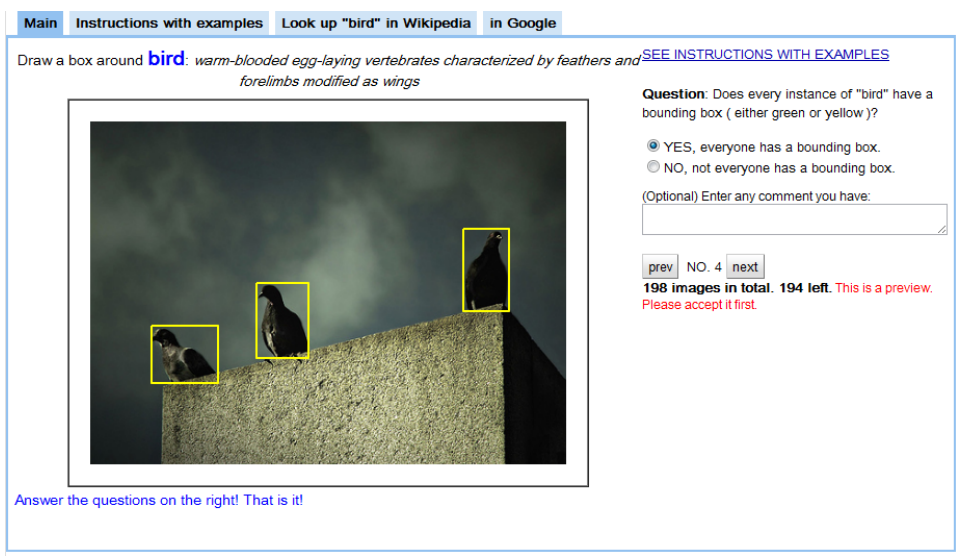
\includegraphics[width=1.0\linewidth]{introduction/crowdsourcing_annotation.jpg}
  \caption{Crowdsourcing image verification task in \cite{Su2012a}} 
  \label{fig:crowdsourcing}
\end{figure}

In this thesis, I use the term Verification Based Annotation (VBA), where machine annotations are checked and verified by a human annotator. Although the idea has played a central role in many previous works, it is not given an easily recognisable term to distinguish it from other kinds of human-in-the-loop machine learning methods such as active learning and is often conflated. A selection of verification based methods are discussed in detail below \cite{Yao2012, McNeill2011, Adhikaria2018, Castrejon2017, Papadopoulos2016, Russakovsky2015a}. 

Verification also plays a large part in ensuring consistency between human annotators in crowdsourcing efforts. The annotations of any one user cannot be fully trusted, and there can be significant variation between annotators. Users are tasked with cross verifying each other's annotations in many of these efforts. An example of a crowdsourcing task \cite{Su2012a} for verifying boxes is shown in Figure~\ref{fig:crowdsourcing}.

Weaker algorithms (machine learning or otherwise) can be used to generate proposals which can then be validated by an annotator. An example of this is in \cite{McNeill2011} where computer vision algorithms generate proposed counts of a penguin colony, and a human operator marks false negatives and false positives.

Human verification is fast; in \cite{Papadopoulos2016}, a yes/no verification is reported as taking 1.6 seconds on average. For a full annotation of a \gls{ILSVRC} image, in \cite{Su2012a} the time to draw a bounding box is reported at 26 seconds (42 seconds after quality control), but \cite{Papadopoulos2017} reports only 7 seconds per box using a more effective input method involving clicking extremities of objects rather than selecting corners. 

\begin{figure}[ht]
  \centering
  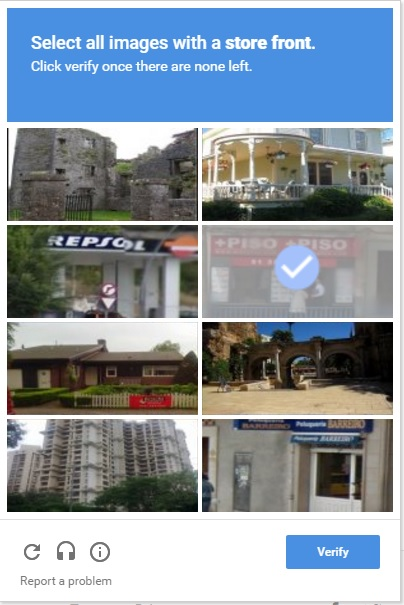
\includegraphics[width=0.5\linewidth]{introduction/recaptcha.jpg}
  \caption{reCAPTCHA dialog showing multi-image verification task}  
  \label{fig:captcha}
\end{figure}

The human ability to verify many examples at once has often been used, for example in the well-known reCAPTCHA \cite{von2008recaptcha}, where one task asks a user to identify objects in a grid of images (shown in Figure~\ref{fig:captcha}). To my knowledge, there is no study confirming if visually validating multiple occurrences together is more efficient than validating single occurrences, but given its extensive use, it seems that this is likely to be the case.

Previous studies on verification based annotation such as \cite{Papadopoulos2016} often focus on localisation for the ImageNet dataset. ImageNet typically features a few large object instances per image (due to its origins as an image classification dataset), with smaller instances often in the background. On domains with many smaller objects such as in biological studies of animals, verifying many instances at once should be much more effective. 

\subsection{Example selection and active learning} 

One prominent human-in-the-loop method is \emph{active learning}. This method revolves around picking the best set of examples for a human to annotate, therefore, making the most effective use of their time. Picking the best examples are often based around an uncertainty measure. Examples, where a model is most uncertain, would often be the most informative examples for learning. 
 
While a \gls{CNN} used for classification provides some measure of uncertainty in its output by interpreting the output from a softmax function as a probability, this is usually not reliable. In \cite{Guo2017} it is shown that modern neural network architectures often systematically overestimate confidence. It is important to find unbiased methods to estimate uncertainty.

\gls{CNN}s with accurate uncertainty measures are still in their infancy, especially for more complex tasks such as object detection. However, recent research has gone into more effectively quantifying uncertainty in \gls{CNN}s with tools such as Bayesian \gls{CNN}s \cite{Gal2017}. Also, other methods of estimating uncertainty have arisen such as ensemble variation \cite{Beluch2018} or mini-batch variation \cite{Chang2017}.

 One recent approach, specific to object detection, is to measure the stability of predicted boxes when noise is added to inputs \cite{Kao2018}. Another idea is to measure consistency between bounding box proposals \cite{Kao2018, Brust2018, Le2018}. Current state-of-the-art object detectors such as \gls{SSD}  \cite{Liu2016a} variants, or \gls{RCNN} \cite{Wang2017} produce a multitude of box proposals where the variation can be measured.

Another measure used in active learning is \emph{expected change}. An example of this is \cite{Vondrick2011} for video annotation, in which frames are selected for annotation that cause large expected changes in the object track. Another example is \cite{Xu2017}, where the expected change is used to measure which parts of a segmentation, if labelled, would cause the most change in the output when using a \gls{CRF}.

Another related but distinct idea is making the best use of the examples available and in the best order. Curriculum learning and self-paced learning \cite{Kumar2010} are research efforts devoted to this goal. Curriculum learning aims to learn from the most informative examples of a dataset to learn faster and more reliably (a recent example is \cite{Katharopoulos2018}). Self-paced learning attempts to have the learning algorithm also determine which examples are hard or easy as it progresses.


\subsection{Semi-supervised learning}

Semi-supervised methods are another active research area which aims to save on annotation time - commonly by either a dataset with only a small portion of labels or a dataset with labels but lacking localisation annotation. Enriching a dataset with localisation information is studied because of the availability of large scale image datasets with class labels. Methods include using the internal activity of a \gls{CNN} to infer the location of objects in an image \cite{Sivic2015}, or consensus forming methods such as \cite{Sangineto} which uses a self-paced learning method beginning with the most reliable examples first, or \cite{Cinbis2017} using multiple data folds to ensure consistency. The latter is used to bootstrap the question-answering verification method \cite{Papadopoulos2016}.

Hard negative and example mining are commonplace in object detection methods to expand a set of annotations unsupervised. Hard negative mining is commonly used in training, where negative examples are not explicitly annotated, yet are necessary to ensure balanced training. In \gls{SSD} \cite{Liu2016a} the training images with the highest confidence non-matching  box proposals are taken as negative examples. An alternative (used in this work) is that of Focal Loss \cite{Lin2017} which samples examples densely and deals with the imbalance by reweighting the loss function. Well classified examples are weighted less, so the bulk of negative examples (which tend to be well classified) do not unbalance the total loss function.

\subsection{Interactive machine learning}

Many human-in-the-loop processes (those that use human refinement to train a learner) are technically a form of interactive machine learning, but more specifically, interactive machine learning uses human inputs to make predictions or directly modify its behaviour.

Interactive machine learning is often used for segmentation where it takes considerable effort to input a segmentation mask, much more than to draw a bounding box, for example. Object selection, for example the GrabCut algorithm \cite{Rother2004}, can be used to find object masks with approximate user input, such as scribbles or bounding box selection. Such a tool can be used iteratively to create, then refine an annotation with the annotator observing the output and making changes to the inputs.  LabelMe \cite{Russell2007} interface provides a scribble based object mask creation tool in this mould. 

\begin{figure}[h]
  \centering
  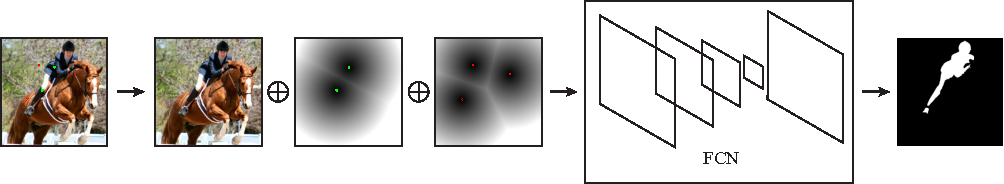
\includegraphics[width=1.0\linewidth]{introduction/object_selection.pdf}
  \caption{Object selection process from \cite{Xu2016}, user input as clicks are turned into distance maps which are concatenated as input to a \gls{FCN} segmentation network}  
  \label{fig:object_selection}
\end{figure}
 
More recently, the same ideas have been applied using \gls{CNN}s where a model can be trained to predict an object mask based on user input, for example, clicks \cite{Xu2016, Boroujerdi2017}, bounding boxes \cite {Xu2017} or extreme points \cite{Maninis2017}. These methods train on datasets containing mask information (without caring about the classes given to the objects), and human input can be simulated based on the mask and bounding box annotations. An illustration of the process from \cite{Xu2016} is shown in Figure~\ref{fig:object_selection}. Human input can also be used to refine an output, for example, in medical segmentation \cite{Wang2017}, or for image colourisation \cite{Zhang} where its primary purpose is to provide a more intuitive editing tool.

A contrasting interactive approach is to have a model provide outputs designed to be easily editable, such as PolygonRNN \cite{Castrejon2017} which provides automatic object selection by bounding box, but provides outputs as a polygon rather than as a mask. The benefit of this approach is that a polygon can be edited more precisely and fed back into training directly.


\subsection {Transfer learning}

Transfer learning is the idea of taking the knowledge gained from a base task and applying it to another. The most prominent and widespread use of transfer learning is perhaps the use of fine-tuning or feature extraction where models trained on classification tasks (typically ImageNet \cite{JiaDeng2009}) are re-purposed for usually much smaller scale tasks in different ways. 

\gls{DECAF} \cite{Donahue2014} showed features extracted from the hidden layers of a \gls{CNN} were directly transferable to achieve the state-of-the-art on many image tasks, including classification and as a much stronger replacement for the handcrafted \gls{SURF} descriptor \cite{bay2006surf}.  Specifically they used AlexNet  \cite{Krizhevsky2012} trained on ImageNet \cite{JiaDeng2009}.

In \cite{Yosinski} it is shown that the transfer-ability of features depends on the distance between the base task to the target task and that using a pre-trained network can even improve generalisation after fine-tuning (as compared to training from scratch).

Fine-tuning retrains a network for a new task, typically using a lower (or zero) learning rate for some parts to preserve the learned weights. 

The use of pre-trained models is now commonplace in adapting \gls{CNN} to new domains, with repositories of state-of-the-art models pre-trained on large datasets existing for most machine learning frameworks (for example the PyTorch \cite{Paszke2017} model zoo). 

Recently, models for visual recognition, such as segmentation or object detection, are usually based around a \emph{backbone} that has previously been trained on a classification task. Examples include the widely used \gls{FPN} network \cite{Lin2017a}, where a base network, for example a ResNet \cite{He} or a DenseNet \cite{Huang2016} backbone which operates from high resolution to low, is combined by a secondary path that operates from low resolution to high with shortcut connections between, combining a pattern seen before in the segmentation U--Net \cite{Ronneberger2015} architecture with pre-trained models.

The \gls{FPN} is now used as a base model in a variety of state-of-the-art segmentation and object detection methods and seems widely applicable to a variety of tasks by attaching a different network \emph{head}, specific to the task at hand (such as classification, or shape regression).

\section {Most related projects to this work}
\label{sec:closest}

\subsection {Interactive object detection \texorpdfstring{\cite{Yao2012}}{}}

Interactive object detection \cite{Yao2012} describes a human-in-the-loop \gls{VBA} system. An incremental object detector (Hough Forest) is trained as a user corrects annotations provided by the system. The focus is placed on minimising the overall annotation cost, in terms of the detection threshold, and then as an active learning measure. 
The cost of annotation time is a linear cost model with factors of: a constant per image, number of false positives, and number of false negatives. The weights for each factor are determined by a short user study, which showed false negatives to be twice as expensive as false positives. 

Active learning is used to select the most difficult images for learning with the highest annotation cost but most informative for learning. The annotation cost is determined from the set of detections, and a model fit using distributions of positive and negative examples from annotations previously verified. 

They evaluate the approach on three datasets with three different example selection methods: incremental image selection (every $n^{th}$ image), active learning, and offline (manual) annotation; demonstrating that both online (\gls{VBA}) methods accelerate annotation, and the active learning method a little better still.

Hough forests \cite{Gall2011}, used as an online learning method are fast to train and fast for inference. They are very suitable for incremental learning because rebuilding the decision trees is fast when image features are pre-computed and can be built after each image is added. 

In comparison, the \gls{CNN} based object detectors used in this work (particularly RetinaNet \cite{Lin2017} and \gls{FPN} \cite{Lin2017a}) require many passes over the training data as the features are learned as part of the training process. The \gls{CNN} detectors benefit from recent developments in object detection and are in general much more capable object detectors. The extra computation required is offset by advances in modern hardware (\gls{GPU}s).

The tools developed in this thesis are a direct successor to this work; however, this connection was not discovered until later in the process. 
Despite the similarities, the focus of each work is different. The annotation tool described in this thesis uses a more sophisticated annotation editor (and the complexities which that entails) as well as tackling practical issues such as its deployment as a web application and use of high-resolution imagery.

One aspect studied in this thesis and not in the earlier work is that of localisation accuracy. Instead of just true positives, false positives and false negatives, there are low confidence detections and poorly localised detections. I attempt to characterise how the object detector's performance relates to annotation time and also how noisy annotation impacts on object detector performance.


\subsection{Fluid Annotation \texorpdfstring{\cite{Andriluka2018}}{}}
\begin{figure}[h]
  \centering
  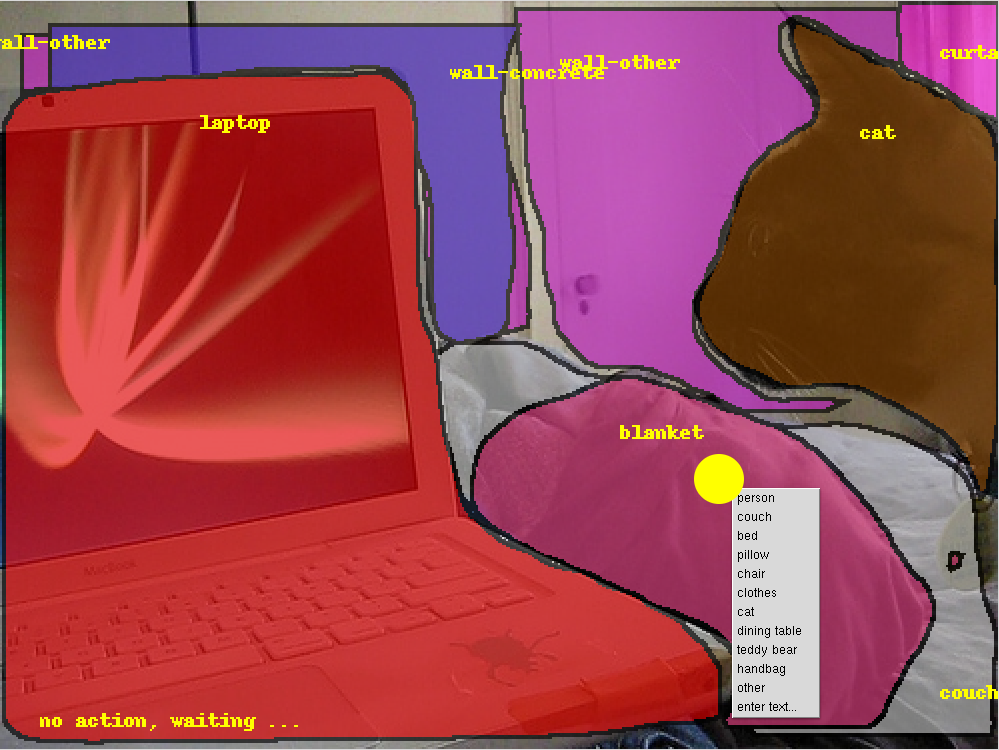
\includegraphics[width=1.0\linewidth]{introduction/fluid_annotation.png}
  \caption{User interface for Fluid Annotation \cite{Andriluka2018}}  
  \label{fig:fluid_annotation}
\end{figure}

Fluid annotation \cite{Andriluka2018} is an interactive human-in-the-loop approach, for instance, to segmentation. The authors point out three key points of their approach, the use of a strong neural network model, editing an entire image at once (as opposed to asking questions about each annotation one by one), and their approach to empower the annotator, rather than employing clever methods to select examples (such as active learning). An example of the user interface is shown in Figure~\ref{fig:fluid_annotation}.

A key difference to my approach is that I focus on annotating and experimentation with new domains, using transfer learning as a tool to enable online learning of the new domain. The strong neural network provides a powerful annotation aid but limits you to annotating images in the same domain as that neural network (which limits the applicability for use in new domains).

\subsection{Faster Bounding Box Annotation for Object Detection in Indoor Scenes  \texorpdfstring{\cite{Adhikaria2018}}{}}

\begin{figure}[h]
  \centering
  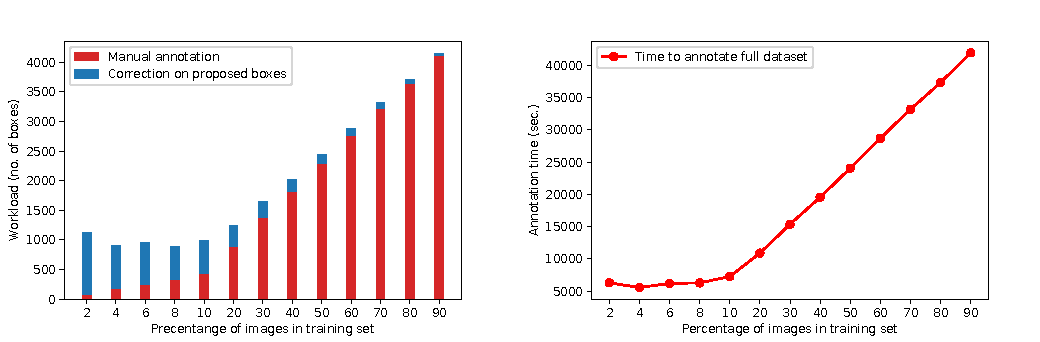
\includegraphics[width=1.0\linewidth]{introduction/adhikaria2018.pdf}
  \caption{Annotation time with different levels of manual annotation vs. assisted annotation. \cite{Adhikaria2018}}  
  \label{fig:adhikaria2018}
\end{figure}

In \cite{Adhikaria2018}, a staged approach to \gls{VBA} is taken. An object detection dataset is annotated in two parts. First, a small dataset split is fully manually annotated and used to train an initial model. Secondly, the remaining data is annotated by having the human annotator verify and refine model predictions. 

One advantage of this staged approach is a more straightforward analysis. Figure~\ref{fig:adhikaria2018} shows the relationship between the number of manually annotated images and the time taken to complete the rest from correcting model predictions.

The work in that study uses a staged approach, and there exists a trade-off between initial annotation effort invested and the accuracy of the detector trained on that initial set. In contrast, the work in this thesis has no staging. By training the model incrementally, the user has the benefit of early model predictions, and yet the model will continue to improve as more images are added.

\subsection {PolygonRNN \texorpdfstring{\cite{Castrejon2017}}{}}

\begin{figure}[h]
  \centering
  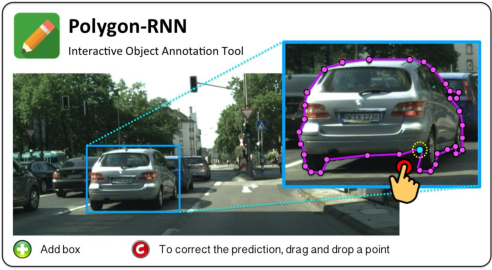
\includegraphics[width=1.0\linewidth]{introduction/polygon_rnn.pdf}
  \caption{The predict and refine process used in PolygonRNN \cite{Castrejon2017}}  
  \label{fig:polygon_rnn}
\end{figure}


Polygon-RNN \cite{Castrejon2017} uses a predict, refine, and train approach in generating segmentation masks (as polygons). A model is trained to segment generic objects, and then it can be fine-tuned for specific tasks. The user first provides a bounding box around an object, the model predicts a polygon and then refines the polygon,  after which it is fed back for training. Figure~\ref{fig:polygon_rnn} illustrates this process, where the user first selects a box around an instance, the model then predicts a sequence of points forming a polygon, and the user then refines those points to better match the true outline.

In this work, I have a very similar goal in Chapter~\ref{chap:bootstrap}, except instead of points I use masks. The advantage of points over masks is better editability and potentially simpler outlines (PolygonRNN has some control in its model over how fine the detail is between points). However, editing with masks also has some advantages: it can provide discontinuous regions and operate without instance recognition. In Chapter~\ref{chap:annotation}, this work focuses on object detection annotation for the whole scene, where PolygonRNN operates on each detected instance. It would be a natural fit to integrate a model like PolygonRNN into the annotation tool developed for this work, and something which may occur in future work.


\subsection {We Don't Need No Bounding Boxes}

\begin{figure}[h]
  \centering
  \includegraphics[width=1.0\linewidth]{introduction/verification.png}
  \caption{Two different kinds of question answering types provided in \cite{Papadopoulos2016}; one simpler with just Yes/No questions (left) and the other more fine-grained (right).}
  \label{fig:verification}
\end{figure}

In \cite{Papadopoulos2016}, a classification dataset is enriched with bounding box information. Instead of annotating a dataset from scratch - a model and dataset are iteratively refined together by asking questions of a human annotator. They initially bootstrap a model using a semi-supervised method  \cite{Cinbis2017} to provide a starting point. A simple Yes/No questioning process is then used to annotate a dataset by refining bounding boxes proposed by the model and intelligently pruning bounding box proposals by adjusting thresholds and overlap (\gls{IOU}). The increase in speed, to achieve nearly equivalent accuracy, is reported at 6 to 9 times.  Figure~\ref{fig:verification} shows an example of the question types.

An advantage of beginning with the weak supervision of image class labels is that it is known that there should be at least one box of that label present. It allows the semi-supervised bootstrapping process. An alternative would be to allow users to draw boxes at the beginning. 

In a similar vein, \cite{Russakovsky2015a} uses a wider variety of interactions with the focus on obtaining a more complete set of annotations, including those too difficult for current object detectors. The tasks include both question asking and manual annotation.


\subsection{Citizen science - Zooniverse \texorpdfstring{\cite{Zooniverse}}{}}

In a later part of this thesis, one of the applications for verification based annotation is counting. This is also a focus for one common use case for the Zooniverse crowdsourcing platform. In \cite{Watson2018} an attempt is made to quantify the success of the Zooniverse platform by showing the amount of data obtained by papers using the platform to be of much greater magnitude than those which don't, and also finds that the citations per paper using data gathered from the platform are much higher. 

One potential advantage of my method over crowdsourcing is consistency. Using a single annotator with assistance from a machine learning model can enjoy the consistency of a single annotator but annotate data at a much faster rate than normal. The downside is potential bias as a result of the machine learning model.

\subsection{ClickBait and ClickBait--v2 \texorpdfstring{\cite{Teng2017, Teng2018}}{}}

ClickBait uses online training to refine an object detector using a human-in-the-loop system and video tracking. Offline training leads to problems with the domain shift in deployment. ClickBait tackles the important idea of refining a visual recognition system online in the field.

A semi-supervised method is used to annotate boxes based on a single click, using the interactive segmentation method of \cite{Xu2016} to segment an object. A bounding box is then placed around the segmentation. In addition, it uses video tracking to track the object across frames. Boxes resulting from these detections can be fed into an online trainer, which is used for tracking a person or vehicle with real-time supervision.


\subsection{BDD100K: A Diverse Driving Video Database with
Scalable Annotation Tooling \texorpdfstring{\cite{Yu2018a} }{}}

As part of the development of the BDD100k dataset \cite{Yu2018a}, an annotation tool was developed, and an experiment performed using a model to initialise bounding box annotations to be verified and adjusted. 

For semi-automated annotation they used a staged approach, using a model trained on $55,000$ annotated video clips. The semi-automated annotation method was compared to a baseline annotation on 2000 image frames and found it took $60\%$ less time.

\subsection{Learning Intelligent Dialogs for Bounding Box Annotation}

\begin{figure}[h]
  \centering
  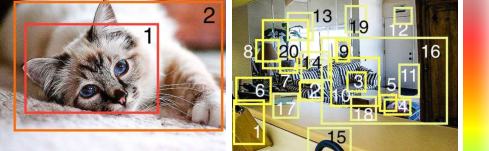
\includegraphics[width=1.0\linewidth]{introduction/intelligent_dialogs.pdf}
  \caption{Two different cases for verifying annotations in an image \cite{Konyushkova2017}. In the first case (left), with two high confidence predictions, a question asking interface is used. In the second case (right) with many low confidence predictions, the user is asked to draw boxes from scratch. }
  \label{fig:intelligent_dialogs}
\end{figure}

Different kinds of annotation tasks can be approached in different ways, and in the case of \gls{VBA}, the best option for having a user verify annotations might not be the same for every image. The focus of \cite{Konyushkova2017} is to intelligently choose the appropriate interface for the image, given the quantity and type of predictions provided by an object detector. At different points in the annotation process, the strength and accuracy of the model means that a different interface might be preferable, even for the same image. An example given is two images (Figure~\ref{fig:intelligent_dialogs}), one with two high scoring predictions, another with many low scoring predictions. To the first, they have a user verify each prediction by answering questions, and the user manually annotates boxes from scratch. To the second the user is asked to draw boxes manually. 


My work also tackles the same issue indirectly (in Chapter~\ref{chap:annotation}). The interface aims to cope with various situations by providing fine control over which object detections are displayed and allowing the user the most flexibility to decide which action to take. In the situation where a user is best to annotate boxes from scratch, the user can make that decision by clearing the existing boxes with a single click. In another situation, many low confidence detections can be dealt with by using a high threshold, thus allowing the user to view and verify low confidence detections by holding down a key. These approaches may not work in all situations, but seem to provide a useful trade-off in many situations.

\subsection {Using DeepLabCut for 3D marker-less pose estimation across species and behaviours \texorpdfstring{\cite{Nath2018, Mathis2018}}{}}

Unlike human pose recognition where there exist some large standardised datasets, there is no such dataset for many applications in tracking wildlife. For these (and other) applications, it is necessary to annotate data. Another more recent work with a similar goal and approach is \cite{Graving2019}.

DeepLabCut is a toolkit for pose estimation, to detect and track custom feature points, building on methods used for human pose estimation. It is provided as a Python toolbox, to be used in an interactive session with a Python interpreter. The user of such a system will use methods from the Python \gls{API} to perform each step. It is a staged \gls{VBA} system with different methods for annotating images (by bringing up a GUI), training models, evaluating new images and then refining those annotations. The steps can then be repeated as necessary to train a pose estimation model and annotate a dataset fully. 

\subsection{Fast and accurate object detection in high resolution 4K and 8K video using GPUs \texorpdfstring{\cite{Ruzicka2018}}{}}

This work details an approach to detecting objects in high-resolution images. They use an attention mechanism first to find areas of interest, then crop overlapping pieces (in a grid) from the high-resolution images for final object detection. Accuracy is improved from 33.6 $AP_{50}$ to 75.4 $AP_{50}$ on one of their internal datasets when comparing the detections from a single down-sampled image to their high-resolution evaluation method. 

The paper describes a similar method to one of the methods investigated in this thesis, where I also crop tiling overlapping regions in the same way. The method described in this thesis does not use an attention mechanism but evaluates all tiling methods. For the image sets in this thesis, I discover that it is possible to use a single evaluation on a simple model instead, with image resolutions much higher than used in training. Using an object detector built around the simple ResNet-18 model, which can already evaluate large images,  I find that the tiling method gives comparable results (see Chapter~\ref{chap:object_detection}).
 
Training is also not described in this paper, it is assumed that the models in use are trained on standard datasets. In this thesis, I show that the object detector can also be trained using crops of high-resolution images. I attempt to characterise the effects of cropping and evaluation at different resolutions, and also find high-resolution evaluation and training to be of significant benefit.
